%\begin{figure}[htb]
%	\centering
%	\fbox{\includegraphics[width = .8\textwidth ]{images/cosmo/cos-part2map-npart.png}}%
%	\caption{
%		The particle distribution of the \cosmo\ dataset.
%		It is a cosmological simulation of $128^3$ dark matter particles at redshift $z=0$ with $H_0 = 70.4$ and density parameters $\Omega_m = 0.272$ and $\Omega_\Lambda=0.728$.
%	}%
%	\label{fig:cosmo_origin}
%\end{figure}




%\begin{figure}[htbp!]
%	\centering
%	\minipage[t]{0.497\textwidth}
%	\centering
%	\fbox{\includegraphics[height=\textwidth]{images/dice-two/dice-two-original-plot.png}}%
%	\caption{
%		The initial particle distribution of the \dt\ dataset. A smaller halo (subhalo 1) made of 40'000 particles is nested within a bigger halo (halo-namegiver), which contains 200'000 particles.
%	}%
%	\label{fig:dice_two_origin}
%	\endminipage%\hspace{.1cm}
%	\hspace*{\fill}
%	%
%	\minipage[t]{0.497\textwidth}
%	\centering
%	\fbox{\includegraphics[height=\textwidth, keepaspectratio]{images/dice-sub/dice-sub-original-plot.png}}%
%	\caption{
%		The initial particle distribution of the \ds\ dataset. 3 small halos (subsubhalo 1-3), made of 20'000 particles, are around a bigger halo (subhalo 1), which contains 200'000 particles. These four structures are then enveloped by an even bigger halo (halo-namegiver), made of 1'000'000 particles.
%	}%
%	\label{fig:dice_sub_origin}
%	\endminipage\hspace*{\fill} 
%\end{figure}


%============================================================================
\subsection{Testing Parameters of the Merger Tree Algorithm}\label{chap:tests}
%============================================================================

%============================================================================
\subsubsection{Methods}
%============================================================================
The current implementation of the merger tree algorithm allows for multiple free parameters for the user to choose from, which will be introduced and tested further below in this section.
Testing these parameters is not a straightforward matter, mainly because there is no ``correct solution'' which would enable a comparison and error quantification.
Nevertheless, one could define a set of quantities one deems a priori favourable for a merger tree and cross-compare these quantities obtained for varying parameters on an identical cosmological simulation.
This method was also used in the ``Sussing Merger Trees Comparison Project'' (\cite{SUSSING_COMPARISON}, \cite{SUSSING_CONVERGENCE}, \cite{SUSSING_HALOFINDER}).
Some or similar quantifications from the ``Sussing Merger Tree'' paper series are adapted in this work, as they seem sensible and even allow for a rough cross-comparison with other merger tree codes.

The following properties will be used to quantify the merger trees:

\begin{itemize}
	\item \textbf{Length of the Main Branch}
	
		The length of the main branch of $z=0$ haloes gives a most basic measure of how far back in time the formation history of these haloes can be tracked.
		Naturally, longer main branches should be considered a favourable feature for a merger tree code.
		
		In this work, the length of the main branch is defined as the number of snapshots a halo and its progenitors appear in.
		A newly formed halo at the $z=0$ snapshot, which doesn't have any progenitors, will by definition have the main branch length of $1$.
		If a halo appears to merge into another, but re-emerges at a later snapshot and is identified to do so, then the snapshots where it is missing from the halo catalogue will still be counted towards the length of the main branch as if it weren't missing. \\

	
	\item \textbf{Branching Ratio}
	
		A further simple tree quantity is the number of branches of the tree.
		The main branch is included in this count, thus the minimal number of branches for each clump at $z=0$ will be $1$.
	
%		Even though the evaluation will be conducted on the identical simulation, some parameters will effect the definitions of haloes an therefore the resulting halo catalogues.
%		As the evaluation will be conducted on the same simulation, I expect lower branching ratios to be accompanied by longer main branches and vice versa.
		As long as the halo catalogue remains unchanged, lower branching ratios mean less merging events and therefore should be accompanied by longer main branches. 
		
		In the picture of bottom-up structure formation, where larger object form through repeated mergers of smaller ones, one would expect more massive clumps to have longer main branches and a higher branching ratio. \\
		
		
	
	\item \textbf{Misidentifications, Quantified by Displacements}
	
		Since no unique correct solution exists, the same displacement statistic $\Delta_r$ as is done in \cite{SUSSING_CONVERGENCE} to quantify misidentifications is used:
%	
		\begin{align}
			\Delta_r = \frac{
				| \mathbf{r}_{k+1} - \mathbf{r}_k - 0.5 (\mathbf{v}_{k+1} + \mathbf{v}_k) (t_{k+1} - t_k) |}
				{0.5(R_{200,k} + R_{200,{k+1}} + | \mathbf{v}_{k+1} + \mathbf{v}_k | (t_{k+1} - t_k)} \label{eq:displacements}
		\end{align}
%
		where $\mathbf{r}_{k+1}$, $\mathbf{v}_{k+1}$ and $\mathbf{r}_k$, $\mathbf{v}_k$ are the position and velocity of a clump at snapshot $k+1$ and its progenitor at snapshot $k$, respectively; $t_{k+1}$ and $t_k$ are the cosmic times at which the two clumps were defined, and $R_{200}$ is the radius that encloses an overdensity of 200 times the critical density $\rho_{c} = \frac{3 H^2}{8 \pi G}$.
		
		It can be interpreted as the difference between the actual displacement $(\mathbf{r}_{k+1} - \mathbf{r}_k)$ and the expected one $(0.5 (\mathbf{v}_{k+1} + \mathbf{v}_k) (t_{k+1} - t_k) )$, normalized by an estimate of how large the displacement is allowed to be to rule out a clear misidentification.
		This estimate is the sum of the average halo size, $0.5(R_{200,k}+R_{200,k+1})$, allowing the exact clump position to vary within its own boundaries, and an estimate for the distance travelled based on the time interval and average velocities, $0.5| \mathbf{v}_{k+1} + \mathbf{v}_k | (t_{k+1} - t_k)$.
		
		Values of $\Delta_r > 1$ would indicate a misidentification, so the parameters minimising $\Delta_r$ should be preferred, provided the acceleration is approximately uniform.
		This is often not the case for subhaloes, which will shift the distribution of $\Delta_r$ towards higher values. 
		Nevertheless, it is used for subhaloes as well, since the goal is a simple cross-comparison of varying parameters, hoping to get some indication towards which parameters produce the most reliable merger trees. \\
		
		
		
		
	\item \textbf{Logarithmic Mass Growth}
	
		The logarithmic mass growth rate of haloes is approximated discretely by
		%
		\begin{align}
			\frac{\de \log M}{\de \log t} \approx \frac{(t_{k+1}+t_{k})(M_{k+1} -M_{k})}{(t_{k+1} - t_k)(M_{k+1} + M_{k})} \equiv \alpha_M(k, k+1)
		\end{align}
		%
		where $k$ and $k+1$ are a clump and its descendant, with masses $M_k$ and $M_{k+1}$ at times $t_k$ and $t_{k+1}$, respectively.
		
		To reduce the range of possible values to the interval $(-1, 1)$, \cite{SUSSING_CONVERGENCE} define
		%
		\begin{align}
			\beta_M = \frac{2}{\pi}\arctan(\alpha_M) \label{eq:massgrowth}
		\end{align}
		%
		Within the hierarchical structure formation scenario, one would expect haloes to grow over time, thus a distribution of $\beta_M$ should be skewed towards $\beta_M > 0$.
        $\beta_M \rightarrow \pm 1$ imply $\alpha_M \rightarrow \pm \infty$, indicating extreme mass growth or losses.\\
		
	\item \textbf{Mass Growth Fluctuations}
		
		Mass growth fluctuations can be quantified by using
		%
		\begin{align}
			\xi_M = \frac{\beta_M(k, k+1) - \beta_M(k-1, k)}{2} \label{eq:massfluct}
		\end{align}
		%
		where $k-1$, $k$, $k+1$ represent consecutive snapshots.
		When far from zero, it implies an extreme growth behaviour. 
        For $\xi_M\rightarrow \pm 1$, $\beta_M(k, k+1) \rightarrow \pm 1$ and $\beta_M(k-1, k) \rightarrow \mp 1$, indicating extreme mass loss followed by extreme mass growth for the upper sign, and the opposite behaviour for the lower sign.
		Within the hierarchical structure formation scenario this behaviour shouldn't occur and such an occurrence might indicate either a misidentification by the tree code or an error in the mass assignment of the halo finder.
\end{itemize}



%In order to produce evaluations that will be comparable to \cite{SUSSING_CONVERGENCE}, only clumps with mass above $5 \cdot 10^{11} \msol$ will be considered for the displacement, mass growth and mass growth fluctuation statistics.
%In all cases that will be considered, more than 3000 clumps have masses above this mass threshold.




In the evaluation, no distinction between main haloes and subhaloes is made.
Distinguishing between those two cases gives no information on which parameters are preferable that can't already be seen when no distinction is made, so for clarity's sake, the evaluations for main haloes and subhaloes individually are omitted from the main body of this work, but the figures for the displacement statistics, logarithmic mass growth and mass growth fluctuations for haloes and subhaloes separately can be found in appendix \ref{app:halo-subhalo-mtree-evals}.
















%============================================================================
\subsubsection{Parameters Influencing the Halo Catalogue}
%============================================================================

In the current implementation, there are two parameters which influence the halo catalogue aside from mass and density thresholds.
The first one concerns the mass definition of a subhalo.
By construction, the mass of a halo contains all its substructure's mass.
This isn't necessarily the case for subhaloes though.
In a hierarchical structure formation scenario, substructures are expected to contain substructures on their own.
Whether to recursively include substructure mass to their respective parent structure is a matter of choice and application. 
The influence of this choice on the merger trees is shown in figures \ref{fig:saddle_nosaddle_masses}, \ref{fig:saddle_nosaddle_mbl_nbranch} and \ref{fig:saddle_nosaddle_displacement}.
When subhaloes' masses are defined to include their respective substructure masses, the results will be labelled as \inc, or \exc\ otherwise.




A second matter of definition is in which case a particle is to be considered as bound to a clump.
The concept of ''exclusively bound`` particles, which aren't allowed to leave the spatial boundaries of their host clump, was introduced in section \ref{chap:unbinding}.
It is to be expected that demanding particles to be exclusively bound will find more unbound particles than not doing so, thus changing the subhalo catalogue.

The influence of this choice on the merger trees is also shown in figures \ref{fig:saddle_nosaddle_masses}, \ref{fig:saddle_nosaddle_mbl_nbranch}, and \ref{fig:saddle_nosaddle_displacement}, along with the influence of the previously described \inc\ and \exc\ mass definitions.
When bound particles are allowed to leave the clump's boundaries, the results will be labelled as \nosad, or \sad\ otherwise.







%============================================================================
\subsubsection{Dataset Used for Testing}
%============================================================================
All tests are performed on the same dark matter only simulation which contains $256^3 \approx 1.7\cdot 10^7$ particles of identical mass $m_p = 1.55\cdot 10^9\msol$. 
The Hubble constant $H_0 = 70.4$ km s$^{-1}$Mpc$^{-1}$ and density parameters $\Omega_m = 0.272$ and $\Omega_\Lambda = 0.728$ were used. 
The density threshold for clump finding was chosen to be 80$\rho_c$  and the saddle threshold for halos was set to 200$\rho_c$, where $\rho_c = \frac{3 H^2}{8 \pi G}$ is the cosmological critical density. 
Only clumps with at least 10 particles were kept.

The output strategy was chosen as follows:
As virtually no haloes were found before $a\leq 0.1$, only few snapshots were stored up to $a=0.1$ in steps of $\Delta a \approx 0.02$.
From this point on, snapshots were created every $\Delta t \approx 0.3$ Gyrs up until $a = \tfrac{1}{3}$, after which a smaller time interval of $\Delta_t \approx 0.2$ Gyrs were chosen.
This choice resulted in 67 snapshots to get to $z = 0$.
The simulation was then continued for 3 further snapshots with $\Delta t \approx 0.2$ Gyrs to ensure that the merging events at $z = 0$ are actually mergers and not clumps that will re-emerge later.

A visualisation of the merger tree of the most massive main halo of this simulation is shown in figure \ref{fig:mergertree}.
Stunningly, even for a relatively low resolution simulation like the one used, incredibly complex formation histories can be uncovered and followed back to the first snapshot with identifiable haloes.
Note that this is only the tree of the central halo, not containing any subhaloes that are still identifiable as such.


\begin{figure}[H]
    \begin{minipage}[c]{0.6\textwidth}
    	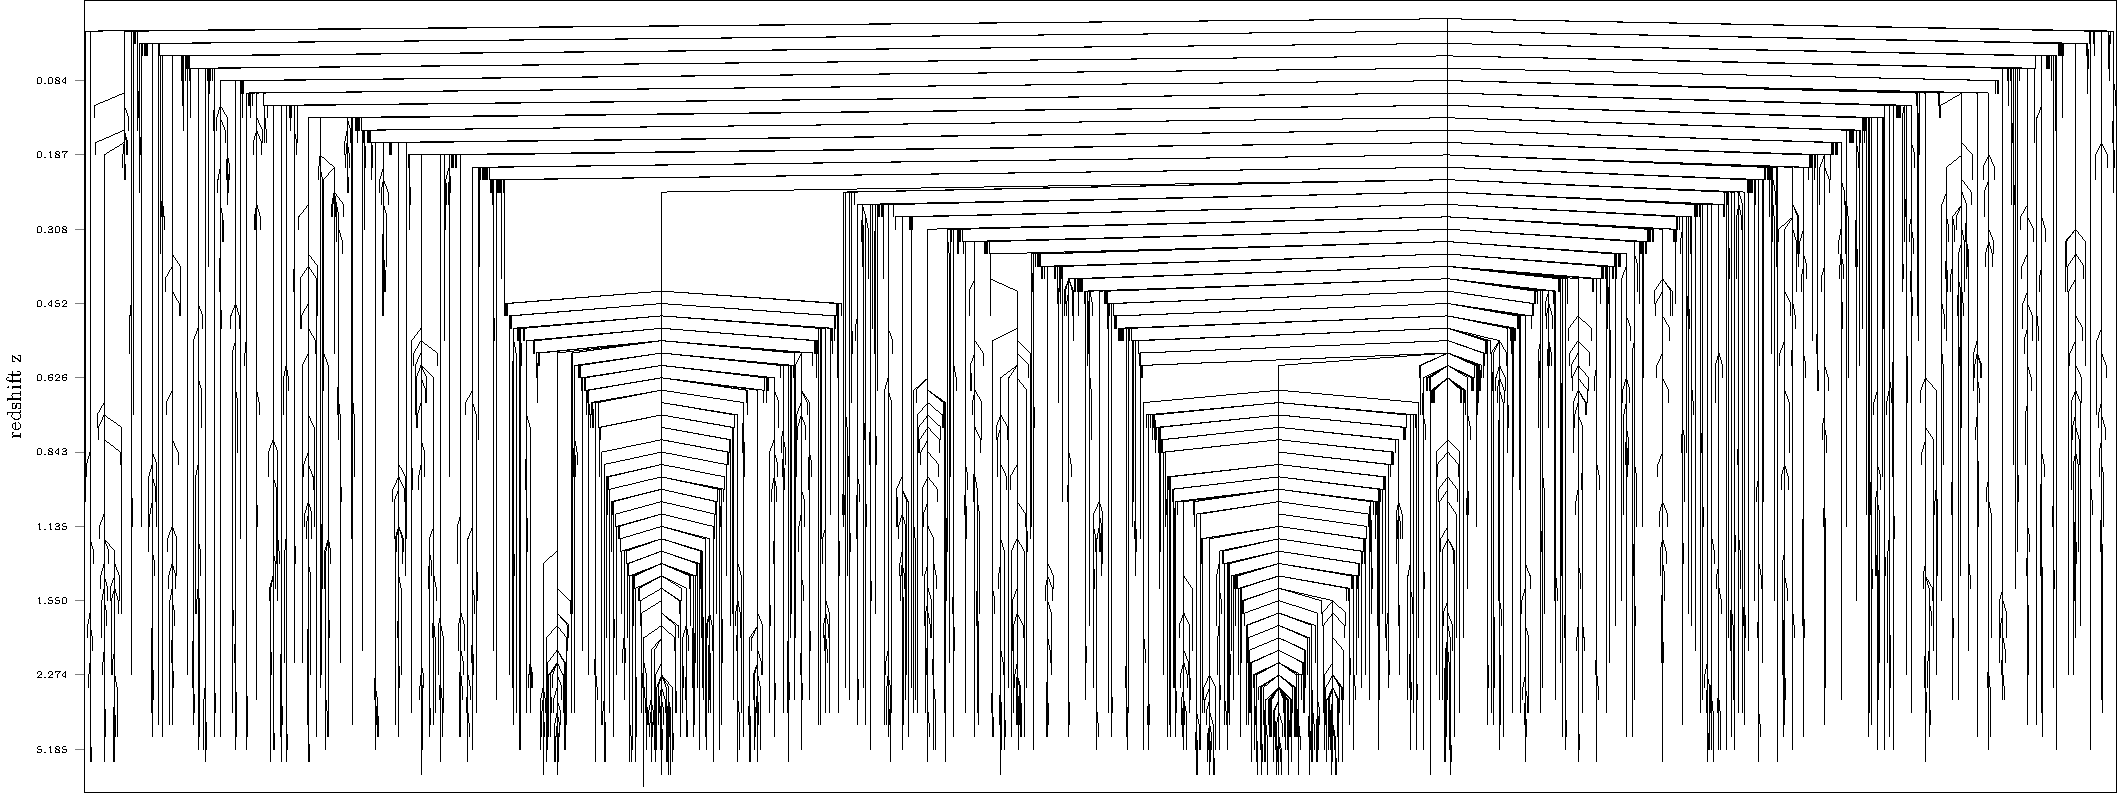
\includegraphics[width=25cm, keepaspectratio,angle=90,origin=c]{images/mergertree.pdf}%
    \end{minipage}\hfill
    \begin{minipage}[c]{0.4\textwidth}
    	\caption{
    		The merger tree of the most massive central halo in the simulation, obtained with the parameters \exc\ and $n_{mb}=1000$.
    		The redshift at the time of the snapshot is given on the $x$-axis, the $y$-axis has no physical meaning.
    	}%
    	\label{fig:mergertree}
    \end{minipage}
\end{figure}









\subsubsection{Influence of the Definition of Subhalo Mass}


\begin{figure}[H]
	\centering
	\includegraphics[width=\textwidth, keepaspectratio]{images/saddle-vs-nosaddle/mass_growth_and_fluctuation.pdf}%
	\caption{
		Logarithmic mass growth and mass growth fluctuation distributions for progenitor - descendant pairs or three consecutive nodes in a branch, respectively, with masses above $5\cdot 10^{11}\msol$ throughout the entire simulation for the halo catalogue influencing parameters: 
		whether subhalo particles are included (\inc) or excluded (\exc) in the clump mass of satellite haloes, and whether to consider particles which might wander off into another clump as bound (\nosad) or not (\sad).
		The distribution is computed as a histogram which is normalised by the total number of events found.
	}%
	\label{fig:saddle_nosaddle_masses}
\end{figure}

\begin{figure}[p]
	\centering
	\minipage[t]{0.49\textwidth}
	\centering
	\includegraphics[width=\textwidth]{images/saddle-vs-nosaddle/length_of_main_branch.pdf}
	\endminipage%\hspace{.1cm}
	\hspace*{\fill}
	%
	\minipage[t]{0.49\textwidth}
	\centering
	\includegraphics[width=\textwidth, keepaspectratio]{images/saddle-vs-nosaddle/number_of_branches.pdf}%
	\endminipage\hspace*{\fill} 
	\caption{
		Length of main branches, defined as the number of snapshots this clump appears in, and the number of branches including the main branch, for the halo catalogue influencing parameters of $z=0$ clumps: 
		whether subhalo particles are included (\inc) or excluded (\exc) in the clump mass of satellite haloes, and whether to consider particles which might wander off into another clump as bound (\nosad) or not (\sad).
		Four distributions are shown, for four different ranges of numbers of particles at $z=0$ exclusively assigned to the clump: less then 100 (top), 100-500, 500-1000 and more than 1000 (bottom), where each particle has mass $m_p = 1.55 \cdot 10^9 \msol$.
		The distribution is computed as a histogram which is normalised by the total number of events found per particle count group.
	}%
	\label{fig:saddle_nosaddle_mbl_nbranch}
\end{figure}

\begin{figure}[H]
	\centering
	\minipage[t]{0.49\textwidth}
		\includegraphics[width=\textwidth]{images/saddle-vs-nosaddle/displacements.pdf}%
		\caption{
			Distribution of the displacements for progenitor - descendant pairs with masses above $5\cdot 10^{11}\msol$ throughout the entire simulation for the halo catalogue influencing parameters: 
			whether subhalo particles are included (\inc) or excluded (\exc) in the clump mass of satellite haloes, and whether to consider particles which might wander off into another clump as bound (\nosad) or not (\sad).
			The distribution is computed as a histogram which is normalised by the total number of events found.
		}%
		\label{fig:saddle_nosaddle_displacement}
	\endminipage%\hspace{.1cm}
	\hspace*{\fill}
	%
	\minipage[t]{0.49\textwidth}
		\centering
		\includegraphics[width=\textwidth]{images/ntracers/displacements.pdf}%
		\caption{
			Distribution of the displacements for progenitor - descendant pairs with masses above $5\cdot 10^{11}\msol$ throughout the entire simulation for varying numbers of clump tracer particles $n_{mb}$.
			The distribution is computed as a histogram which is normalised by the total number of events found.
		}%
		\label{fig:ntracers_displacement}
	\endminipage
\end{figure}













%===============================================================
%\subsubsection*{Length of Main Branch and Branching Ratio}
%===============================================================

\begin{table*}
	\caption{
        Average data for all clumps at $z=0$ depending on whether to consider particles which might wander off into another clump as bound (\nosad) or not (\sad).
        The results shown are for the \exc\ mass definition, which show no significant difference to when the \inc\ mass definition is used.
%        The groups I, II, III and IV are defined as clumps that contain less then 100, 100-500, 500-1000 or more than 1000 particles, respectively.
        \label{tab:saddle_nosaddle}
    }
        
%	{\small 
%		\begin{tabular}[c]{l | p{2.8cm} | p{2.8cm} |}
%													&	 \sad\  &   \nosad\ \\ 
%			
%			\hline
%			%
%			total clumps	 						&	 16262	& 	17242 	\\			
%			%		
%%			max number of particles in a clump 		&	 414570	& 	271438 	\\			
%			%		
%			median number of particles in a clump 	&	 83		& 	93 		\\			
%			%
%			\hline
%			%		
%			average main branch length group I		&	23.153	& 	20.527 	\\			
%			%
%			average main branch length group II		&	48.835	& 	48.642 	\\			
%			%		
%			average main branch length group III	&	54.715	& 	54.904 	\\			
%			%
%			average main branch length group IV		&	53.958	& 	56.265 	\\			
%			%
%			\hline
%			%		
%			average number of branches group I		&	1.327	& 	1.230 	\\			
%			%
%			average number of branches group II		&	3.448	& 	3.603 	\\			
%			%		
%			average number of branches group III	&	8.670	& 	8.661 	\\			
%			%
%			average number of branches group IV		&	29.457	& 	28.607 	\\				
%			%
%			\hline	
%		\end{tabular}
%	}

	{\small 
		\begin{tabular}[c]{l | p{2.8cm} | p{2.8cm} |}
													&	 \sad\  &   \nosad\ \\ 
			
			\hline
			%
			total clumps	 						&	 16262	& 	17242 	\\			
			%		
%			max number of particles in a clump 		&	 414570	& 	271438 	\\			
			%		
			median number of particles in a clump 	&	 83		& 	93 		\\			
			%
			\hline
			%
			average main branch length & & \\
			%	
			clumps with < 100 particles		&	23.2	& 	20.5 	\\			
			%
			clumps with 100-500 particles	&	48.8	& 	48.6 	\\			
			%		
			clumps with 500-1000 particles	&	54.7	& 	54.9 	\\			
			%
			clumps with > 1000 particles	&	54.0	& 	56.3 	\\			
			%
			\hline
			average number of branches & & \\
			%		
			clumps with < 100 particles		&	1.3		& 	1.2 	\\			
			%
			clumps with 100-500 particles	&	3.4		& 	3.6 	\\			
			%		
			clumps with 500-1000 particles	&	8.7		& 	8.7 	\\			
			%
			clumps with > 1000 particles	&	29.5	& 	28.6 	\\				
			%
			\hline	
		\end{tabular}
	}
\end{table*}

In accordance to the hierarchic structure formation picture, more massive clumps tend to have longer main branches and a higher branching ratio in all cases.
This is clearly visible from the average length of the main branch and the average branching ratio of clumps at $z=0$, binned in four groups by their mass, which are given in table \ref{tab:saddle_nosaddle}.
The average main branch length for clumps with more that 500 particles is $\sim 55$, meaning that on average, haloes with mass above $\sim 7.75 \cdot 10^{11} \msol$ can be traced back to redshift $\sim 3$.

The length of the main branches for the same four mass bins of clumps are shown in figure \ref{fig:saddle_nosaddle_mbl_nbranch}.
Interestingly, small clumps with less than 100 particles seem to have a somewhat constant formation rate from $z \sim 2$ until $z \sim 0.2$.
Furthermore they too can be traced back to high redshifts, indicating good performance of the merger tree algorithm.

Whether subhalo masses are computed in an \exc\ or \inc\ manner seems to have negligible effect on the branching ratio and the length of main branch.

The \sad\ definition of bound particles however tends to result in longer main branch lengths for small clumps with less than 100 particles.
This might be explained by the fact that in general, when \sad\ is applied, subhaloes which are at the bottom of the clump hierarchy will tend to contain less bound particles compared to when \nosad\ is used, and have shorter lifetimes because they are found to have merged into their hosts earlier.
Therefore clumps with more than 100 particles with the \nosad\ condition might be moved to the lower mass bin of $\leq$ 100 particles when \sad\ is used, thus increasing the fraction of clumps with high main branch lengths (lengths of 50-60), as well as the number of branches.
Evidence of the earlier merging can be seen in the overall higher number of branches in the right column of figure \ref{fig:saddle_nosaddle_mbl_nbranch}, as well as the average values, total clump numbers and the median particle numbers in a clump given in table \ref{tab:saddle_nosaddle}.
%The longer main branch length can be understood by considering that with a clump definition which in general has less particles, some clumps which would otherwise be sorted in a higher mass bin are sorted in a lower one instead.
%This should increase both the length of main branches and the number of branches for lower mass clumps (below 100 particles) and decrease them for high mass clumps (above 1000 particles), as table \ref{tab:saddle_nosaddle} and figure \ref{fig:saddle_nosaddle_mbl_nbranch}.
%For intermediate masses, meaning 100-1000 particles in a clump, the distributions and average values don't vary significantly.








%==========================================
%\subsubsection*{Misidentifications}
%==========================================

The displacement statistic used to quantify misidentifications in figure \ref{fig:saddle_nosaddle_displacement} indicates that no parameter choice results in a obviously ``wronger'' progenitor-descendant pairing.
Even though there are some  $\Delta_r > 1$, indicating that there might be misidentifications present, it can't be determined easily whether they truly are.
When the displacement statistic is calculated for haloes and subhaloes separately, which is shown in appendix \ref{app:halo-subhalo-mtree-evals}, no halo descendant-progenitor pair shows a displacement above 1, indicating no obvious misidentifications, yet a significant fraction of subhalo progenitor-descendant pairs have a high displacement value $\Delta_r > 1$.
However, the displacement statistic is calculated assuming a uniform acceleration, which is not valid for subhaloes.
On the other hand, the fact that any parameter pair used found at least some clumps with more than 1000 particles at $z=0$ with main branch length of unity, which is the case when it doesn't have any progenitor, and thus essentially ``appearing out of nowhere'', is strongly suggesting present misidentifications.




%=========================================================================
%\subsubsection*{Logarithmic Mass Growth and Mass Growth Fluctuations}
%=========================================================================

The logarithmic mass growth in figure \ref{fig:saddle_nosaddle_masses} shows that as expected, the distribution is indeed skewed towards $\beta_M > 0$. 
When the \inc\ parameter is used, the distribution of mass growth contains a few more extreme mass growths and losses $(\beta_M \rightarrow \pm 1)$, as well as some high mass growth fluctuations $(\xi_M \rightarrow \pm 1)$ (see figure \ref{fig:saddle_nosaddle_masses}).
When the \nosad\ parameter is used, noticeably more extreme mass growth $(\beta_M \rightarrow \pm 1)$ and mass growth fluctuations $(\xi_M \rightarrow \pm 1)$ occur.






%==========================================
%\subsubsection*{Conclusion}
%==========================================
In conclusion, whether to use \inc\ or \exc\ mass definitions for subhaloes shows very little effect on the merger trees.
Based on the fewest extreme mass growth fluctuations, the \sad\ parameter is clearly preferable. 
%With \sad\ in use, the \exc\ parameter leads to less clumps over 1000 particles with main branch length of 1, and a little fewer extreme mass growths and fluctuations, which is why I conclude that the combination of \exc\ and \sad\ parameters should create the most reliable merger trees.





	













%===================================================================
\subsection{Influence of the Number of Tracer Particles Used}
%===================================================================

\begin{table}[ht]
	\begin{center}
		{\small 
		\begin{tabular}[c]{l | p{1cm} | p{1cm} | p{1cm} | p{1cm} | p{1cm} | p{1cm} | p{1cm} |}
			$n_{mb}=$								&	1 		& 	10 		& 	50 		& 	100 	& 200 	& 500 		& 1000 \\
			\hline
	%
%			total clumps at $z=0$					&	16262	& 	16262	& 	16262	&	16262 	& 16262  & 16262 	& 16262 \\
	%		
%			max NoP in a clump 		&	414570	& 	414570	& 	414570	&	414570 	& 414570 & 414570 	& 414570  \\ 	
	%		
%			median NoP in a clump 	&	83		& 	83		& 	83		&	83  	& 83	 & 83 	& 	83  \\	
	%
%			\hline
	%		
			average MBL group I		&	24.188	& 	24.330	& 	23.567	&	23.353 	& 23.153 & 22.876 	& 22.656  \\	
	%
			average MBL group II		&	50.399	& 	50.116	& 	49.472	&	49.122 	& 48.835 & 48.777 	& 48.762  \\	
	%		
			average MBL group III	&	55.233	& 	54.863	& 	53.264	&	54.059 	& 54.715 & 54.327 	& 54.165  \\	
	%
			average MBL group IV		&	56.690	& 	54.884 	& 	52.345	&	52.900 	& 53.958 & 55.761 	& 56.448  \\
	%
			\hline
	%		
			average NoB group I		&	1.228	& 	1.305	& 	1.296	&	1.305 	& 1.327  & 1.357 	& 1.367  \\	
	%
			average NoB group II		&	2.699	& 	3.062	& 	3.265	&	3.337 	& 3.448  & 3.586 	& 3.596  \\	
	%		
			average NoB group III	&	6.625	& 	7.229	& 	8.051	&	8.206 	& 8.670  & 8.914 	& 9.121  \\	
	%
			average NoB group IV		&	20.407	& 	25.237	& 	27.288	&	28.554 	& 29.457 & 30.443 	& 31.420  \\	
	%
			\hline	
		\end{tabular}
		}
	\caption{
		Average data for all clumps at $z=0$ for varying numbers of clump tracer particles $n_{mb}$. 
		The groups I, II, III and IV are defined as clumps that contain less then 100, 100-500, 500-1000 or more than 1000 particles, respectively.
		``MBL'' is an abbreviation for ``main branch length'', ``NoB'' stands for ``number of branches''.
        % ``NoP'' for ``number of particles''.
		}
	\label{tab:ntracers}
	\end{center}	
\end{table}
\begin{table}[ht]
	\begin{center}
		{\small 
		\begin{tabular}[c]{l | p{1cm} | p{1cm} | p{1cm} | p{1cm} | p{1cm} | p{1cm} | p{1cm} |}
			$n_{mb}=$								&	1 		& 	10 		& 	50 		& 	100 	& 200 	& 500 	& 1000  \\
			\hline	
			trees pruned from tree catalogue		&	33924	&	23091	&	22146	& 	22131 	& 22130 & 22129 & 22129 \\	
	%
			highest particle number of a LIDIT		&	1369	&	236		&	236		&	236 	& 236 	& 157 	& 157  	\\	
	%
			median particle number of a LIDIT		&	19		&	20		&	20		&	20 		& 20 	& 20 	& 20  	\\
	%
			LIDITs with >100 particles pruned 		&	513		&	42		&	32		&	26 		& 25 	& 24 	& 24  	\\
    %
            total number of jumpers                 &  20176    &   20905   &   22074   &   22041   & 20970 & 19307 & 18249 \\
			\hline
		\end{tabular}
		}
	\caption{
		Trees pruned from the merger tree catalogue for varying numbers of clump tracer particles $n_{mb}$ throughout all snapshots. 
		``LIDIT'' is an abbreviation of ``last identifiable descendant in tree''. 
		For LIDITs no further descendants could be identified throughout the simulation and consequently their tree was pruned from the merger tree catalogue.
        A ``jumper'' refers to a clump that has been merged into another clump at some snapshot, but re-emerged at a later snapshot, like shown in figure \ref{fig:jumper-demo}.
		}
	\label{tab:ntracers-pruning}
	\end{center}	
\end{table}

\begin{figure}[H]
	\centering
	\includegraphics[width=\textwidth, keepaspectratio]{images/ntracers/mass_growth_and_fluctuation.pdf}%
	\caption{
		Logarithmic mass growth and mass growth fluctuation distributions for progenitor - descendant pairs or three consecutive nodes in a branch, respectively, with masses above $5\cdot 10^{11}\msol$ throughout the entire simulation for varying numbers of clump tracer particles $n_{mb}$.
		The distribution is computed as a histogram which is normalised by the total number of events found.
	}%
	\label{fig:ntracers_masses}
\end{figure}

\begin{figure}[p]
	\centering
	\minipage[t]{0.49\textwidth}
	\centering
	\includegraphics[width=\textwidth]{images/ntracers/length_of_main_branch.pdf}
	\endminipage%\hspace{.1cm}
	\hspace*{\fill}
	%
	\minipage[t]{0.49\textwidth}
	\centering
	\includegraphics[width=\textwidth, keepaspectratio]{images/ntracers/number_of_branches.pdf}%
	\endminipage%\hspace*{\fill}
	\caption{
		Length of main branches, defined as the number of snapshots this clump appears in, and the number of branches including the main branch of $z=0$ clumps for varying numbers of clump tracer particles $n_{mb}$.
		Four distributions are shown, for four different ranges of numbers of particles at $z=0$ exclusively assigned to the clump: less then 100 (top), 100-500, 500-1000 and more than 1000 (bottom), where each particle has mass $m_p = 1.55 \cdot 10^9 \msol$.
		The distribution is computed as a histogram which is normalised by the total number of events found per particle count group.
	}%
	\label{fig:ntracers_mbl_nbranch}
\end{figure}













%===================================================================
%\subsubsection*{Length of Main Branch and Branching Ratio}
%===================================================================

The average number of branches and average main branch lengths are shown in table \ref{tab:ntracers}.
The average number of branches increases with the number of tracers used, the case for $n_{mb}=10$ for clumps with less than 100 particles being the only exception.
The average main branch length decreases for the two lower mass clump bins (less than 500 particles).
This can also be seen in the top two rows of figure \ref{fig:ntracers_mbl_nbranch}, where the length of the main branches and the number of branches are plotted.
This indicates that more mergers were detected.
Counter-intuitively, this can be seen as a sign that more reliable trees are created with increasing $n_{mb}$.
Recall that progenitors from adjacent snapshots are given priority over non-adjacent ``jumpers''.
By tracking more particles per clump, more candidates can be expected to be found, which is supported by the fact that the number of jumpers in the simulations decreasing with increasing $n_{mb}$ (see table \ref{tab:ntracers-pruning}).
Considering that also being a main progenitor to any descendant is given priority over being merged into the main descendant of the progenitor, it should be safe to say that it should be true merging events that have been misidentified by tracking fewer $n_{mb}$ particles.
%A contributing factor might be that with more tracers, more progenitor-descendant links of adjacent snapshots are made and less connections across multiple snapshots are necessary, reducing the risk of assigning the wrong formation history across multiple snapshots.
%However, since direct progenitors from adjacent snapshots are given priority to non-adjacent ones, misidentifications might just as well be introduced by this behaviour.
%Table \ref{tab:ntracers-pruning} also shows that for $n_{mb}>100$, the total number of connections across multiple snapshots (``jumpers'') starts to decrease.

When a clump has no descendant candidates at all, its tree is removed from the list of trees.
How many of these trees have been pruned throughout the simulation is shown in table \ref{tab:ntracers-pruning}, as well as the particle number of the most massive pruned clump, the median particle number of pruned clumps and the number of clumps containing more than 100 particles that have been pruned.
With increasing $n_{mb}$, the number of pruned clumps, the highest particle number of a pruned clump, and the number of clumps with more than 100 particles decreases.
Notice that for $n_{mb}=1$, there is a drastic increase in all these three quantities.
In particular, clumps with more than 1000 particles are pruned, meaning that haloes with mass above $1.5\cdot 10^{12} \msol$ simply vanished between two snapshots.
These statistics indicate furthermore that with increasing number of tracing particles, more merging events are detected.









%===============================================
%\subsubsection*{Misidentifications}
%===============================================
The displacements in figure \ref{fig:ntracers_displacement} show virtually no differences.
The only noticeable difference is towards the high end of $\Delta_r$, where $n_{mb}=1$ and $n_{mb}=10$ have a small peak further out than the other choices for $n_{mb}$.










%====================================================================
%\subsubsection*{Logarithmic Mass Growth and Mass Growth Fluctuations}
%====================================================================
The logarithmic mass growth and mass growth fluctuations in figure \ref{fig:ntracers_masses} show that these distributions mostly overlap, but extreme growths $(\beta_M \rightarrow \pm 1)$ and fluctuations $(\xi_M \rightarrow \pm 1)$ decrease with increasing $n_{mb}$.






%===============================================
%\subsubsection*{Conclusion}
%===============================================

It seems that $n_{mb} = 100-200$ is a good compromise between computational efficiency and good results.
Note that for this simulation, the median number of particles in $z=0$ clumps was 83, meaning that with $n_{mb} = 100$, more than half of identified clumps were being tracked by every particle they contain.













\subsection{Outlook}

Based on the previously shown results, the current implementation of the merger tree algorithm seems to perform well.
The shapes of the logarithmic mass growths and mass growth fluctuations in figures \ref{fig:saddle_nosaddle_masses} and  \ref{fig:ntracers_masses} as well as the distributions of lengths of main branches and number of branches are in good agreement with the results from other merger tree codes, which have been compared in \cite{SUSSING_HALOFINDER}. 
However, there are still some unanswered conceptual questions and possible algorithm optimisations to be discussed.

On the conceptual side, when linking progenitors and descendants across multiple snapshots, one must ask:
How far in the future or in the past does one need to look for a descendant or progenitor, respectively?
At what point should one assume that the tracked progenitor is really dissolved and definitely won't reappear at later times?
The current implementation only contains the option to forget past merged progenitors after a user defined number of snapshots has passed, but by default, it will track them until the simulation ends.
By not removing orphans at all and using them to link descendants with progenitors across multiple snapshots, misassignments are enabled, leading to wrong formation histories.

Two possible solutions would be the following:

\begin{enumerate}
    \item Estimate the time a clump would require to completely merge into its parent structure, after which the progenitor shouldn't be tracked anymore. This is for example done in \cite{Moster}, where they compute the dynamical friction time $t_{df}$ of a merged subhalo based on the orbital parameters found at the last snapshot where this subhalo was identified:
    \begin{equation}
        t_{df} = \alpha_{df} \frac{V_{vir} r_{sat}^2}{G M_{sat}\ln \Lambda} \label{eq:dynamical_friction_time}
    \end{equation}
    where $r_{sat}$ is the distance between the centres of the main halo and of the subhalo, $M_{sat}$ is the mass of the subhalo, $\ln\Lambda = (1 + M_{vir}/M_{sat})$ is the Coulomb logarithm, $M_{vir}$ is the virial mass of the main halo, $V_{vir}$ is the circular velocity of the main halo at the virial radius and $\alpha_{df} = 2.34$. 
    A smaller subhalo inside a main halo experiences dynamical friction because of its gravitational attraction: 
    At any given moment, it attracts the particles of the host towards the point in space where it currently resides, but because the subhalo itself is in orbit, it will move away from that point, thus leaving a slightly denser trail along the path it moves.
    The gravitational attraction from this trail on the other hand will eventually slow it down and cause it to fall into the main halo's centre.
    
    Another possibility would be to use the fitting formula for the merger timescale of galaxies in cold dark matter models by \cite{merger_timescales}.
    
    
    \item The particle used to track a past merged progenitor is also the same particle that an orphan galaxy is assigned to.
    In principle, it should be possible to define some galaxy merging cross-sections such that the probability of a collision between an orphan galaxy and a non-orphan galaxy which will result in a galaxy merger can be computed.
    Unknown parameters of these cross-sections should be able to be calibrated using N-body simulations.
    After a collision, one could remove the orphan from future snapshots.
\end{enumerate}



From a technical viewpoint, one clear bottleneck in the current merger tree algorithm is the requirement to write progenitor particles and data to file and read them back in and sort them out at a later snapshot.
An elegant solution would be to permanently store the clump IDs of particles in memory, however this would require an extra integer per particle in the simulation, which becomes prohibitively expensive for large simulations not only because it would need a lot of memory, but also because more data needs to be communicated between MPI tasks.

An option would be to track which particles left each task's domain and which particles entered between two snapshots.
The clump IDs of particles would still be read and written to and from files, but it would minimise the sorting part of the algorithm where each MPI task figures out which tracker particles it contains.
The necessary data of particles that left or entered new domains between snapshots could then be communicated with one collective MPI communication, provided they've been tracked in a clever manner.

Another option would be to change the amount of data each MPI task needs to read in.
Currently, every MPI task reads in and writes to one shared file using MPI reading and writing routines in order to maximally make use of the parallel architecture.
Instead, each task could write its own file.
Meanwhile, between snapshots, the maximal velocity of any particle should be traced.
This way, once the simulation advances to the next snapshot, it would be possible to estimate the maximal distance any particle could've travelled.
Provided every MPI task has knowledge on how the entire computational domain is split between tasks, it could skip reading in data written by tasks where no particle currently in this task's domain could have come from.
This would however probably require a more sophisticated communication for progenitor data such as their mass or descendant candidates.
(Currently, because every MPI task reads in all the progenitor data, this communication are simple collective scatter and gather operations.)
Furthermore, the situation will get more complicated if the domain decomposition changes its shape between snapshots to e.g. load balance.





%Dynamical friction plays a crucial role in the formation and
%evolution of galaxies. During the merger of two dark matter halos,
%galaxies in a less massive halo will become the satellite galaxies of
%the more massive one. These satellite galaxies gradually lose their
%energy and angular momentum under the action of dynamical
%friction and are predestined to sink to the center of the massive
%dark matter halo if they are not disrupted by the tidal force.
%Dynamical friction takes effect through interaction of galaxies
%with background dark matter particles. Chandrasekhar (1943) gave
%a description of this phenomenon for an idealized case where a
%rigid object moves through a uniform sea of collisionless matter
%particles. This description can be applied to the case of a satellite
%galaxy moving in a dark matter halo. The orbits of dark matter
%are deflected by the galaxy, which produces an enhancement of
%dark matter density behind the galaxy. Consequently, the galaxy
%suffers a steady deceleration by the drag of the wake and will
%eventually merge to the central galaxy of the dark matter halo.
%The merger timescale, i.e., the time elapsing between entering
%the virial radius of the dark matter halo and final coalescence of
%satellite and central galaxy, can be derived using Chandrasekhar’s
%formula (see, e.g., Binney & Tremaine 1987). In addition, taking
%into account the dependence on the orbital circularity, Lacey &
%Cole (1993) derived the following expression for the merger time-
%scale of a satellite galaxy orbiting around a massive halo with
%circular velocity



